\paragraph{Example 1}
\begin{lstlisting}[language=Python]
from BNumMet.Visualizers.InterpolationVisualizer import InterpolVisualizer
interpolVisualizer = InterpolVisualizer()
display(interpolVisualizer.run())
\end{lstlisting}
\begin{enumerate}
\item Initial State: \\
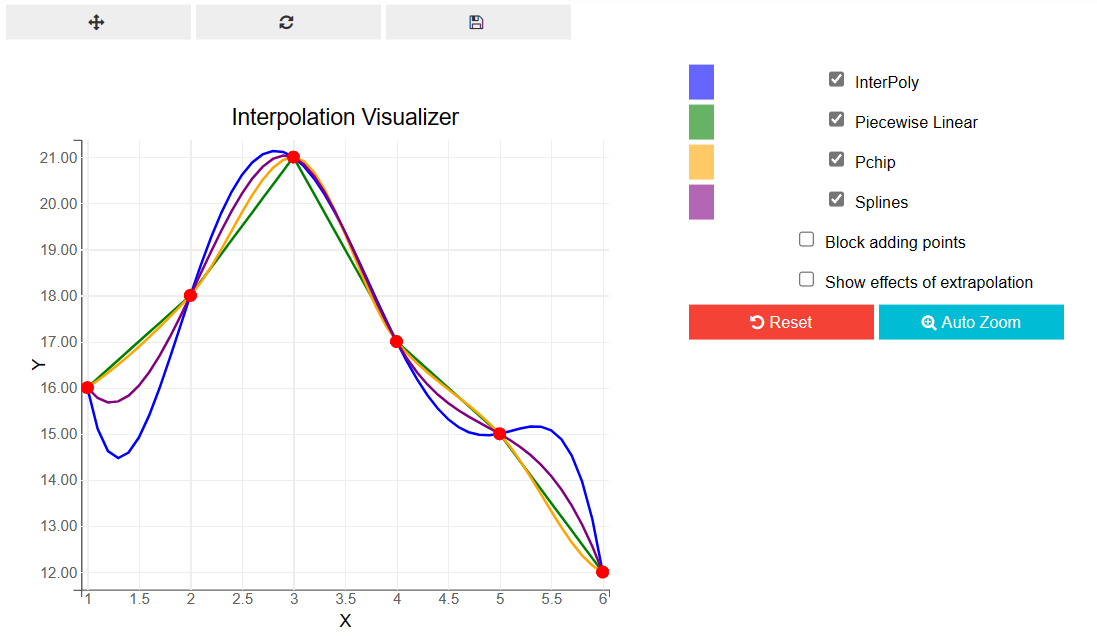
\includegraphics[scale=0.5]{Include/Images/Thesis/Documentation/Visualizers/Interpolation/Example 1/Example 1 - 00 - Initial State.png}

\item Checked Box Extrapolation and AutoZoom: \\
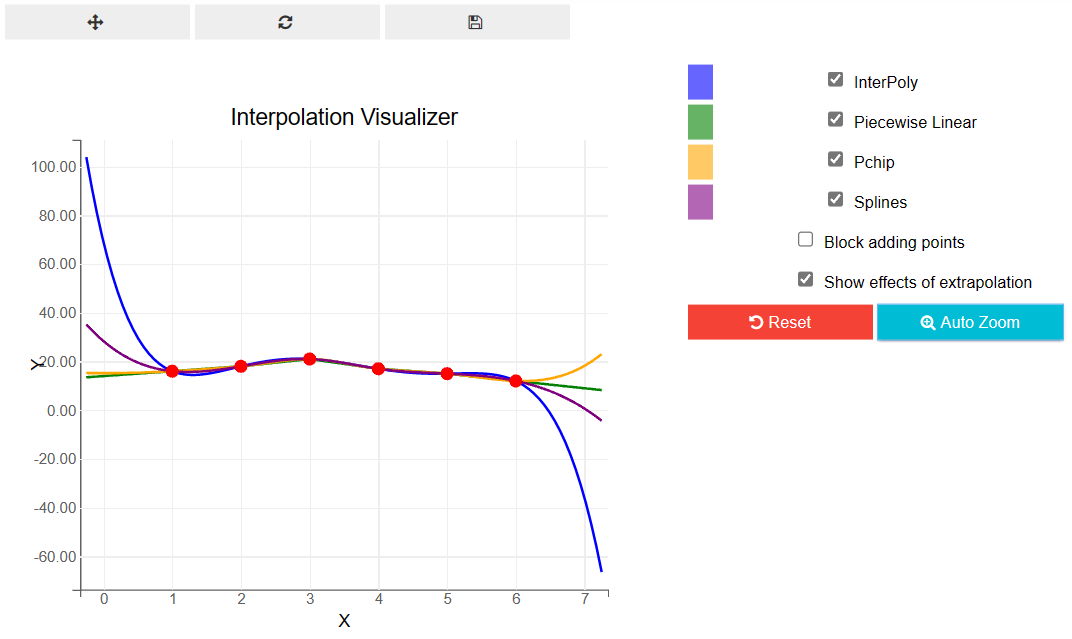
\includegraphics[scale=0.5]{Include/Images/Thesis/Documentation/Visualizers/Interpolation/Example 1/Example 1 - 01 - Checked Box Extrapolation and AutoZoom.png}

\item Reset Button: \\
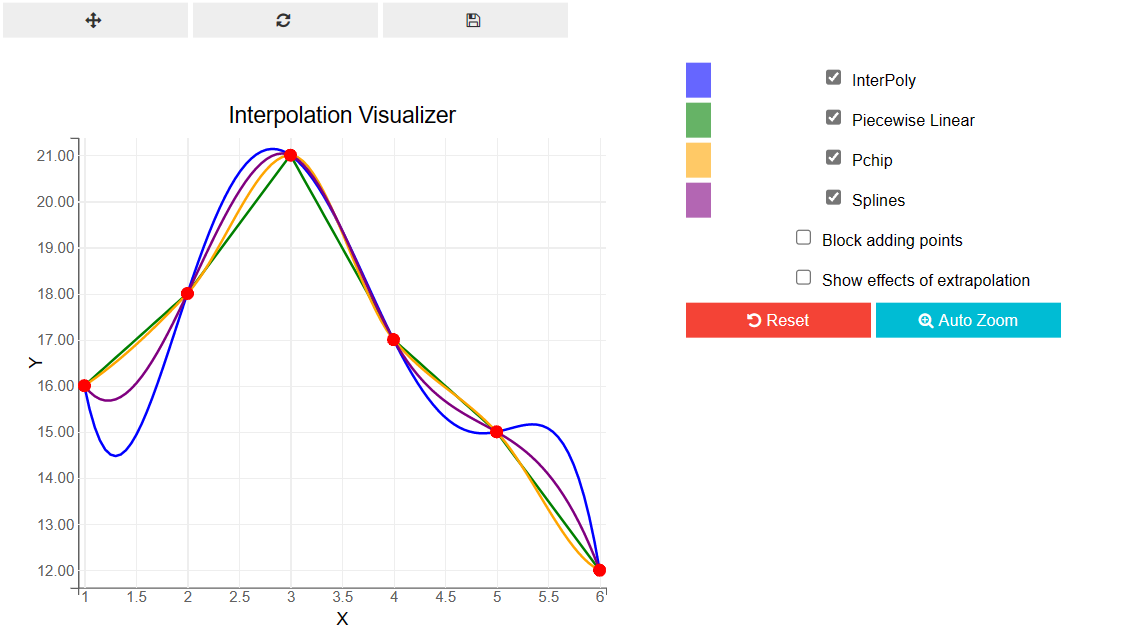
\includegraphics[scale=0.5]{Include/Images/Thesis/Documentation/Visualizers/Interpolation/Example 1/Example 1 - 02 - Reset Button.png}

\item Added Point: \\
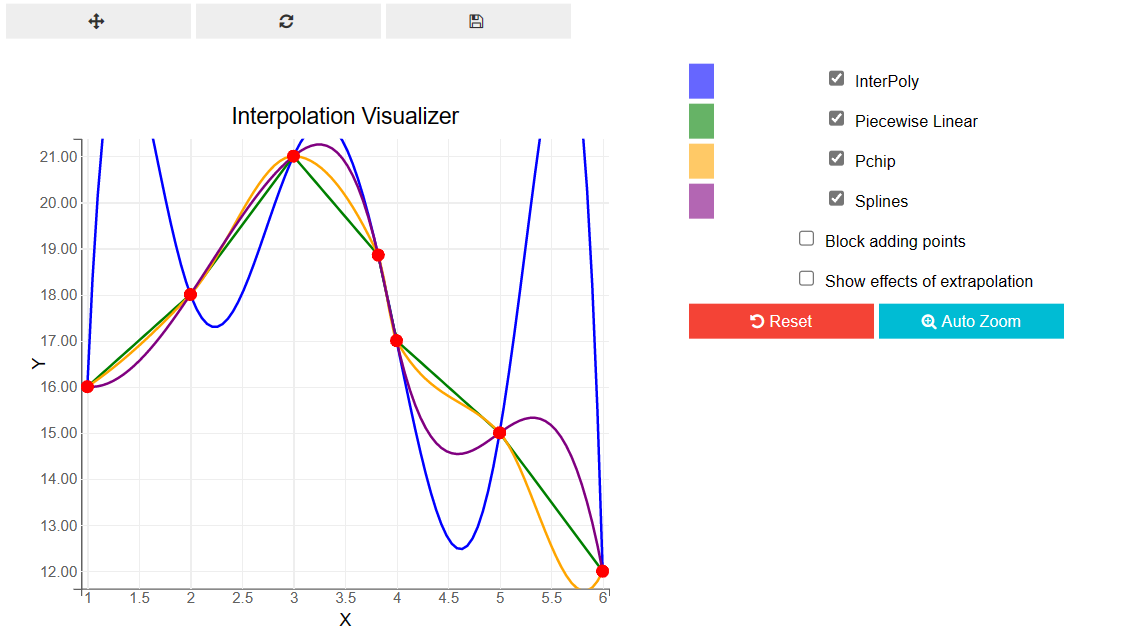
\includegraphics[scale=0.5]{Include/Images/Thesis/Documentation/Visualizers/Interpolation/Example 1/Example 1 - 03 - Added Point.png}

\item AutoZoom: \\
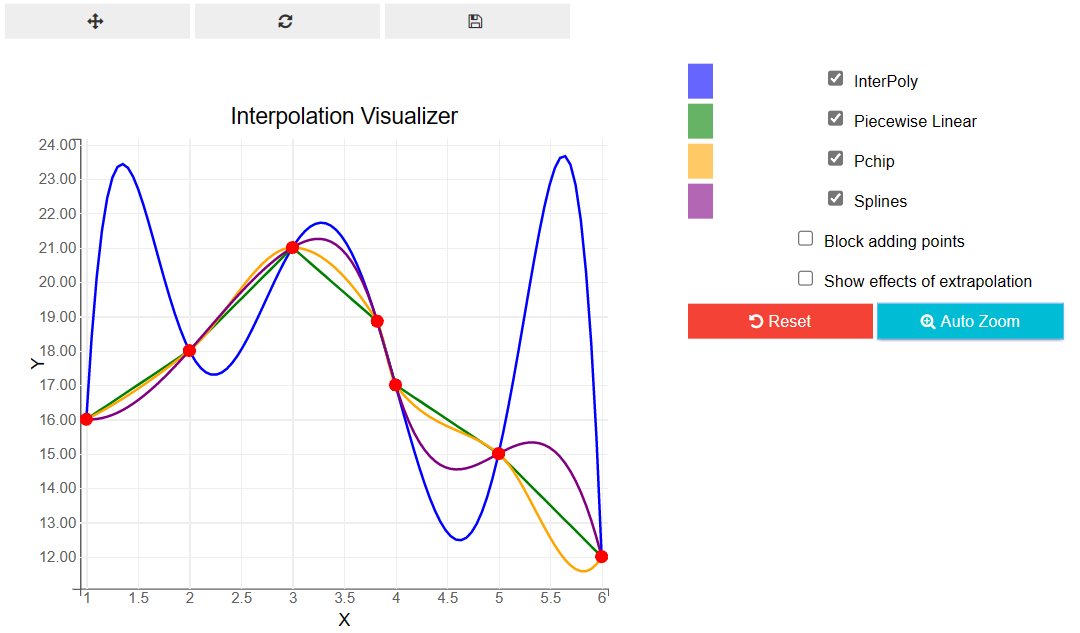
\includegraphics[scale=0.5]{Include/Images/Thesis/Documentation/Visualizers/Interpolation/Example 1/Example 1 - 04 -AutoZoom.png}
\end{enumerate}